%%%%%%%%%%%%%%%%%%%%%%%%%%%%%%%%%%%%%%%%%
% Beamer Presentation
% LaTeX Template
% Version 1.0 (10/11/12)
%
% This template has been downloaded from:
% http://www.LaTeXTemplates.com
%
% License:
% CC BY-NC-SA 3.0 (http://creativecommons.org/licenses/by-nc-sa/3.0/)
%
%%%%%%%%%%%%%%%%%%%%%%%%%%%%%%%%%%%%%%%%%{}

%----------------------------------------------------------------------------------------
%	PACKAGES AND THEMES
%----------------------------------------------------------------------------------------
%%%%%%%%%%%%%%%%%%%%%%%%%%%%%%%%%%%%%%%%%
% Modified By Orcuslc, 2016-9-21
% Modified for Assignments
% http://github.com/orcuslc
%
% Wilson Resume/CV
% Structure Specification File
% Version 1.0 (22/1/2015)
%
% This file has been downloaded from:
% http://www.LaTeXTemplates.com
%
% License:
% CC BY-NC-SA 3.0 (http://creativecommons.org/licenses/by-nc-sa/3.0/)
%
%%%%%%%%%%%%%%%%%%%%%%%%%%%%%%%%%%%%%%%%%

%----------------------------------------------------------------------------------------
%	PACKAGES AND OTHER DOCUMENT CONFIGURATIONS
%----------------------------------------------------------------------------------------
\documentclass[10pt]{article}

\usepackage{listings}
\usepackage{xcolor}
\usepackage{amsmath,amsthm,amssymb}
\usepackage{epstopdf}
\usepackage{graphicx}
\usepackage{clrscode3e}

\DeclareGraphicsExtensions{.eps,.ps,.jpg,.bmp}


\usepackage[a4paper, hmargin=25mm, vmargin=30mm, top=20mm]{geometry} % Use A4 paper and set margins

\usepackage{fancyhdr} % Customize the header and footer

\usepackage{lastpage} % Required for calculating the number of pages in the document

\usepackage{hyperref} % Colors for links, text and headings

\setcounter{secnumdepth}{0} % Suppress section numbering

%\usepackage[proportional,scaled=1.064]{erewhon} % Use the Erewhon font
%\usepackage[erewhon,vvarbb,bigdelims]{newtxmath} % Use the Erewhon font
\usepackage[utf8]{inputenc} % Required for inputting international characters
\usepackage[T1]{fontenc} % Output font encoding for international characters

\usepackage{fontspec} % Required for specification of custom fonts
\setmainfont[Path = ./fonts/,
Extension = .otf,
BoldFont = Erewhon-Bold,
ItalicFont = Erewhon-Italic,
BoldItalicFont = Erewhon-BoldItalic,
SmallCapsFeatures = {Letters = SmallCaps}
]{Erewhon-Regular}

\usepackage{color} % Required for custom colors
\definecolor{slateblue}{rgb}{0.17,0.22,0.34}

\usepackage{sectsty} % Allows customization of titles
\sectionfont{\color{slateblue}} % Color section titles

\fancypagestyle{plain}{\fancyhf{}\cfoot{\thepage\ of \pageref{LastPage}}} % Define a custom page style
\pagestyle{plain} % Use the custom page style through the document
\renewcommand{\headrulewidth}{0pt} % Disable the default header rule
\renewcommand{\footrulewidth}{0pt} % Disable the default footer rule

\setlength\parindent{0pt} % Stop paragraph indentation

% Non-indenting itemize
\newenvironment{itemize-noindent}
{\setlength{\leftmargini}{0em}\begin{itemize}}
{\end{itemize}}

% Text width for tabbing environments
\newlength{\smallertextwidth}
\setlength{\smallertextwidth}{\textwidth}
\addtolength{\smallertextwidth}{-2cm}

\newcommand{\sqbullet}{~\vrule height .8ex width .6ex depth -.05ex} % Custom square bullet point 


\newcommand{\tbf}[1]{\textbf{#1}}
\newcommand{\tit}[1]{\textit{#1}}
\newcommand{\mbb}[1]{\mathbb{#1}}
\newcommand{\blue}[1]{\color{blue}{#1}}
\newcommand{\red}[1]{\color{red}{#1}}
\newcommand{\sblue}[1]{\color{slateblue}{#1}}
\newcommand{\n}{\\[5pt]}
\newcommand{\tr}{^\top}
\newcommand{\vt}[1]{
\Vert #1 \Vert
}
\newcommand{\bra}[5]{
#1=\left\{
\begin{aligned}
#2 ,&\quad #4 \\
#3 ,&\quad #5
\end{aligned}
\right.
}

\renewcommand{\title}[2] {
{\Huge{\color{slateblue}\textbf{#1}}}
\hfill
\LARGE{\color{slateblue}\textbf{#2}} \\[10pt]
\large{\color{slateblue}\textbf{Chuan Lu, 13300180056, chuanlu13@fudan.edu.cn}} \\[1mm]
\rule{\textwidth}{0.5mm}
}

\newcommand{\problem}[2] {
\vspace{20pt}
\LARGE{\color{slateblue}\textbf{Problem #1.}}
\vspace{2mm}
#2 \\[10pt]
}

\renewcommand{\proof}[2] {
\large{\color{slateblue}\textit{\textbf{#1.}}}
#2 \qed \\[3mm]
}

\newcommand{\solution}[2] {
\large{\color{slateblue}\textit{\textbf{#1.}}}
#2 \\[3mm]
}


\newcommand{\algorithm}[2] {
\begin{codebox}
\Procname{$\proc{Algorithm #1}$}
#2
\end{codebox}
}

\newcommand{\refgroup}[1] {
\LARGE{\color{slateblue}\textbf{Reference}} 
\begin{tabbing}
\hspace{5mm} \= \kill
#1
\end{tabbing}
}

\newcommand{\reference}[1] {
\sqbullet \ \  \large{#1} \\
}
% \newcommand{\solution}[2] {
% \LARGE{\color{slateblue}\textit{#1}}
% \ #2 \qed
% }

% \newenvironment{problem}[2][Problem]{\begin{trivlist}
% \item[\hskip \labelsep {\bfseries #1}\hskip \labelsep {\bfseries #2.}]}{\end{trivlist}}

\mode<presentation> {

% The Beamer class comes with a number of default slide themes
% which change the colors and layouts of slides. Below this is a list
% of all the themes, uncomment each in turn to see what they look like.

\usetheme{default}
% \usetheme{AnnArbor}
% \usetheme{Antibes}
% \usetheme{Bergen}
% \usetheme{Berkeley}
% \usetheme{Berlin}
% \usetheme{Boadilla}
% \usetheme{CambridgeUS}
% \usetheme{Copenhagen}
% \usetheme{Darmstadt}
% \usetheme{Dresden}
% \usetheme{Frankfurt}
% \usetheme{Goettingen}
% \usetheme{Hannover}
% \usetheme{Ilmenau}
% \usetheme{JuanLesPins}
% \usetheme{Luebeck}
% \usetheme{Madrid}
% \usetheme{Malmoe}
% \usetheme{Marburg}
% \usetheme{Montpellier}
% \usetheme{PaloAlto}
% \usetheme{Pittsburgh}
% \usetheme{Rochester}
% \usetheme{Singapore}
% \usetheme{Szeged}
% \usetheme{Warsaw}

% As well as themes, the Beamer class has a number of color themes
% for any slide theme. Uncomment each of these in turn to see how it
% changes the colors of your current slide theme.

%\usecolortheme{albatross}
%\usecolortheme{beaver}
%\usecolortheme{beetle}
%\usecolortheme{crane}
%\usecolortheme{dolphin}
%\usecolortheme{dove}
%\usecolortheme{fly}
% \usecolortheme{lily}
%\usecolortheme{orchid}
%\usecolortheme{rose}
%\usecolortheme{seagull}
%\usecolortheme{seahorse}
%\usecolortheme{whale}
%\usecolortheme{wolverine}

%\setbeamertemplate{footline} % To remove the footer line in all slides uncomment this line
%\setbeamertemplate{footline}[page number] % To replace the footer line in all slides with a simple slide count uncomment this line

%\setbeamertemplate{navigation symbols}{} % To remove the navigation symbols from the bottom of all slides uncomment this line
}

\usepackage{graphicx} % Allows including images
\usepackage{booktabs} % Allows the use of \toprule, \midrule and \bottomrule in tables
\usepackage{xeCJK}
\usepackage{algorithm,algpseudocode, algorithmicx}
%\usepackage{algorithmic}
\usepackage{float} %算法浮动体

%----------------------------------------------------------------------------------------
%	PACKAGE SETTINGS
%----------------------------------------------------------------------------------------

\floatname{algorithm}{算法}

%\setCJKmainfont[BoldFont={黑体-简}, ItalicFont={楷体-简}]{宋体-简}
%%\setCJKmainfont{宋体}
%\setCJKsansfont[BoldFont={黑体-简}, ItalicFont={楷体-简}]{宋体-简}
%%\setCJKsansfont{宋体}
%\setCJKmonofont[BoldFont={黑体-简}, ItalicFont={楷体-简}]{宋体-简}
%%\setCJKmonofont{宋体}

%\AtBeginSection[]
%{
%\begin{frame}
%\tableofcontents[currentsection,hideallsubsections]
%\end{frame}
%}

%----------------------------------------------------------------------------------------
%	TITLE PAGE
%----------------------------------------------------------------------------------------

\title[SVR in Load Prediction]{SVR in Load Prediction} % The short title appears at the bottom of every slide, the full title is only on the title page

\author{Chuan Lu, Fudan University} % Your name
\institute[Fudan]
{} % Your institution as it will appear on the bottom of every slide, may be shorthand to save space
% {
% \large{Fudan University} \\ % Your institution for the title page
% % \medskip
% % \textit{cqfu13@fudan.edu.cn} % Your email address
% }
\date{Nov 11, 2016} % Date, can be changed to a custom date

\begin{document}

\begin{frame}
\titlepage % Print the title page as the first slide
\end{frame}

\begin{frame}
\frametitle{Outline} % Table of contents slide, comment this block out to remove it
\tableofcontents % Throughout your presentation, if you choose to use \section{} and \subsection{} commands, these will automatically be printed on this slide as an overview of your presentation
\end{frame}

%----------------------------------------------------------------------------------------
%	PRESENTATION SLIDES
%----------------------------------------------------------------------------------------

%------------------------------------------------

\section{Goal}
\begin{frame}
\frametitle{Goal}
To predict the max load of the following 1/3/7,... days with information we can get from history data and/or forecast of the next days.
\end{frame}

\section{SVR} % Sections can be created in order to organize your presentation into discrete blocks, all sections and subsections are automatically printed in the table of contents as an overview of the talk
\begin{frame}
\frametitle{SVR}
\begin{block}{From Wikipedia:}
SVR is a version of Support Vector Machine (SVM) used for regression, proposed by Vladimir N. Vapnik in 1996. It is a supervised learning method, equivalent to solving
$$minimize\quad \frac{1}{2}\vt{w}^2$$
$$subject\ to \both{y_i - <w, x_i> - b\leq \varepsilon}{<w, x_i>+b-y_i\leq \varepsilon}$$
\end{block}
\end{frame}

\begin{frame}
\frametitle{SVR}
It can be used to do linear or unlinear regressions using the support vectors, especially when the characters of data are linearly non-separable. In this case we can use different kernels to map data points into a higher-dimensional space. The most commonly used kernel is Gaussian Kernel (or called Radial Basis Function)
$$K(x, x_c) = e^{-\frac{\vt{x-x_c}^2}{2\sigma^2}}$$
\end{frame}

%%------------------------------------------------
\section{Parameters Selection}
\begin{frame}
\frametitle{Parameters}
In the given dataset, the only useful information is the dependent variable \textbf{load}.
But from publications we can find many other parameters which could be used in our model.
\end{frame}

\begin{frame}
\frametitle{Parameters}
\begin{itemize}
\item MAX Load of yesterday
\item MAX Load of 3, 5, 7, ... days before
\item Weather information: temperature, wind speed/direction, humidity, ...
\item Calendar information: weekends, weekday, holiday, ...
\item Special Case: G20 summit, Regulation, ...
\item ...
\end{itemize}
\end{frame}

\begin{frame}
\frametitle{Parameters in practical use}
After Cross-Validation, we finally chose the following parameters:
\begin{itemize}
\item MAX Load of past 6 days (Scaled: Divided by 10000)
\item Temperature of tomorrow (Scaled: Divided by 29)
\item Calendar info: Weekdays (By 6 Bi-digits), Holidays (By -1, 0, 1)
\end{itemize}
\end{frame}

\section{Details in Code}
\begin{frame}
\frametitle{Dependency}
Written and Tested By Python 3.5. We wish the module could be deployed in Linux-based systems.
\begin{itemize}
	\item Python 3+ (3.4+ preferred)
	\item Python-numpy (The latest version)
	\item Python-scipy
	\item Python-scikit-learn
	\item Python-pandas
	\item Python-matplotlib
\end{itemize}
\end{frame}

\begin{frame}
\frametitle{Usage}
See Readme.html
\end{frame}

\section{Results in Forecast}
\begin{frame}
\frametitle{Prediction Result}
\begin{figure}
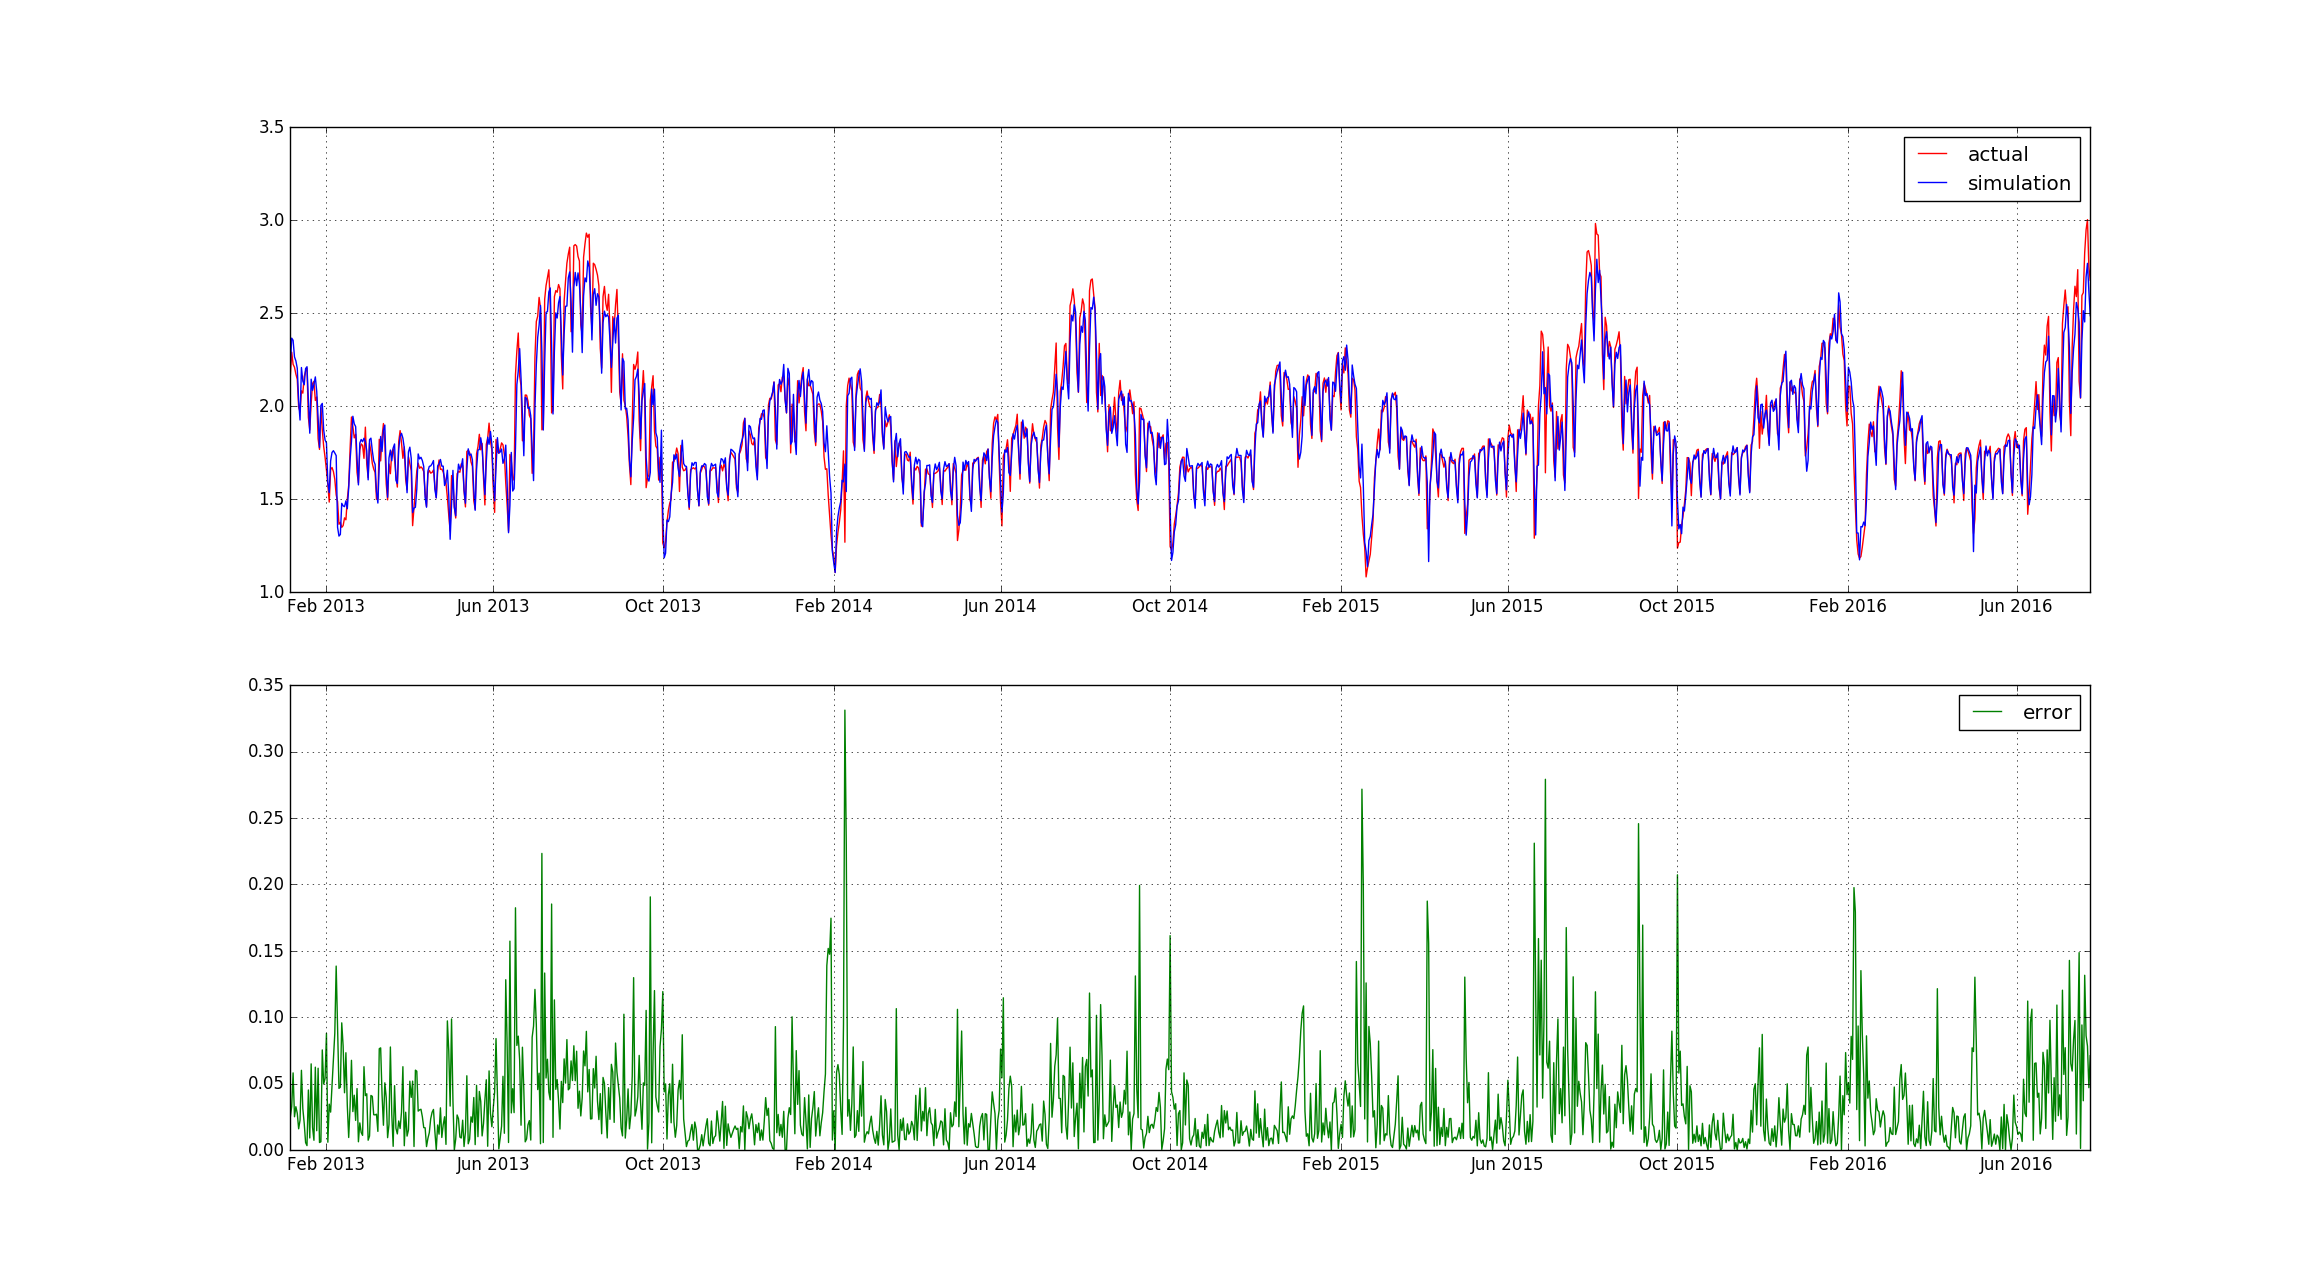
\includegraphics[width=\textwidth]{img/Pred.png}
\end{figure}
\end{frame}

\begin{frame}
\frametitle{Conclusion}
Use 2 years' data as training set, 3.5 years' data as testing set.s
\begin{itemize}
	\item Total average error is 3.1\%.
	\item MAX error is 33\%.
	\item Those over 20\% are almost caused by holidays.
	\item The prediction is somehow too convergent.
\end{itemize}
\end{frame}

\begin{frame}
\frametitle{Conclusion}
There are some points for further study and improvement:
\begin{itemize}
	\item Holidays could be marked artificially, we can adjust simply by multiplying a constant.
	\item We can bind the results of different methods, for example, Kalman Filters always produce radical results and SVR produce moderate ones; If we use the average of these two methods, there could be a more accurate one.
\end{itemize}
\end{frame}
%%------------------------------------------------

%%------------------------------------------------



%%------------------------------------------------


%----------------------------------------------------------------------------------------

\end{document}